\chapter{Tinh chỉnh mô hình hội thoại trên máy cá nhân}
\section{Mục tiêu và phạm vi}
Các câu hỏi thử cho thấy phản hồi theo mẫu còn cứng và dễ thiếu bối cảnh. Nhánh hội thoại cục bộ bổ sung Qwen3 1.7B để diễn đạt kiến thức lấy từ KB. Mô hình nền đã được Qwen tiền huấn luyện; thực nghiệm này chỉ tinh chỉnh LoRA trên ví dụ tiếng Việt của project. Việc tải mô hình không được tính là một lần huấn luyện.

Suy luận diễn ra trên máy cá nhân, không gọi dịch vụ mô hình ngôn ngữ bên ngoài. Bản Vercel tiếp tục phục vụ KB, luật và các mô hình dữ liệu bảng; checkpoint Qwen không chạy trong hàm Vercel. Hai chế độ dùng chung giao diện nhưng có điều kiện vận hành khác nhau.
\section{Dữ liệu và thiết kế đánh giá}
\subsection{Nguồn và cách xây dựng}
Tệp \path{experiments/local_qwen/dataset.json} chứa các cặp chỉ dẫn và phản hồi do project biên soạn từ các đoạn KB có nguồn. Mỗi mẫu lưu câu hỏi, lịch sử, mã đoạn kiến thức và câu trả lời đích. Nguồn KB gồm các tài liệu sức khỏe đã liệt kê trong danh mục. Đây không phải dữ liệu bệnh án và chưa được chuyên gia y tế thẩm định.

Tập huấn luyện gồm 76 mẫu; tập validation gồm 21 mẫu diễn đạt khác nhưng cùng nguồn KB. Tập test gồm 16 mẫu, chia đều thành nhóm kiến thức và nhóm hội thoại. Kiểm tra chuẩn hóa câu hỏi loại trùng lặp trực tiếp giữa các tập. Tuy vậy, cùng nguồn và cùng cách biên soạn làm giới hạn tính độc lập của đánh giá. Hai nhóm test không được gọi là hai bộ dữ liệu lâm sàng độc lập.
\subsection{Đối chiếu trước và sau tinh chỉnh}
Mô hình nền và checkpoint LoRA nhận cùng tài liệu, câu hỏi, lịch sử và giới hạn sinh. Chọn checkpoint bằng loss validation, không dùng điểm test để chọn epoch. Nhóm kiến thức kiểm tra trả lời đúng trọng tâm và dẫn mã nguồn; nhóm hội thoại kiểm tra thông tin thiếu, câu hỏi tiếp nối, lời cảm ơn, yêu cầu thuốc và câu ngoài phạm vi. Loss giảm chỉ cho thấy mô hình khớp câu trả lời đích tốt hơn; không đủ kết luận độ chính xác y tế tăng.
\section{Cấu hình và quá trình học}
Máy thực nghiệm có Intel Core i9-14900HX, RAM khoảng 16 GB và NVIDIA GeForce RTX 4060 Laptop GPU 8 GB. Mô hình nền được tải từ kho chính thức:
\productlink{Qwen3 1.7B}{https://huggingface.co/Qwen/Qwen3-1.7B}

LoRA giữ cố định trọng số nền $W$ và học hai ma trận nhỏ để tạo $W'=W+\frac{\alpha}{r}BA$. Cấu hình dùng hạng $r=8$, $\alpha=16$, dropout 0,05, áp dụng vào các phép chiếu query và value. Hàm mất mát chỉ tính trên token câu trả lời, bỏ qua phần chỉ dẫn và tài liệu.

Batch size bằng 1 nghĩa là một mẫu được xử lý trong mỗi lượt lan truyền; tích lũy gradient qua 4 mẫu trước khi cập nhật. Một epoch đi qua toàn bộ tập train. AdamW cập nhật tham số từ gradient với learning rate $10^{-4}$. Thực nghiệm đặt 3 epoch, tối đa 768 token cho một mẫu, dùng BF16 và gradient checkpointing để giảm bộ nhớ. Training loss theo bước và validation loss theo epoch được lưu riêng để theo dõi khả năng khái quát hóa.
\subsection{Kết quả đo trên máy thực nghiệm}
Số tham số được tối ưu là 1,605,632, trên tổng 1,722,180,608 tham số. Checkpoint được chọn ở epoch 3. Loss validation của mô hình nền là 1.0810; giá trị tốt nhất sau tinh chỉnh là 0.0082. Thời gian ba epoch, gồm đánh giá validation và lưu checkpoint, là 1.97 phút. Bộ nhớ GPU cấp phát đỉnh do PyTorch ghi nhận là 3.93 GiB; số này không bao gồm toàn bộ bộ nhớ các ứng dụng khác.
\begin{figure}[htbp]\centering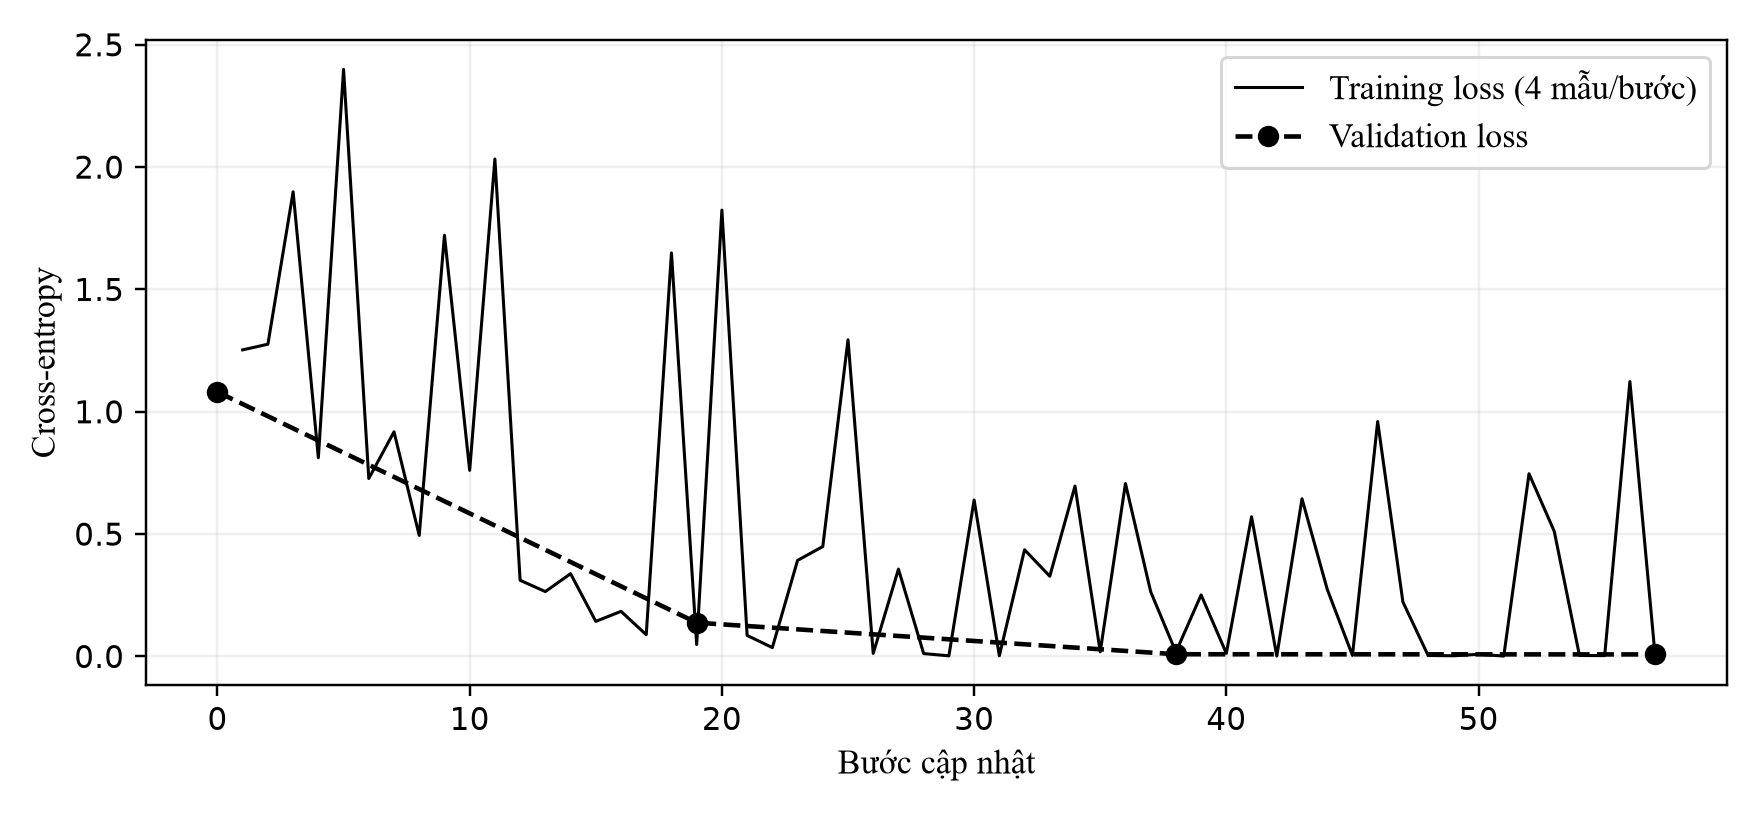
\includegraphics[width=\linewidth]{figures/qwen_learning.png}\caption{Loss huấn luyện theo bước và validation theo epoch. Điểm đầu validation thuộc mô hình nền.}\end{figure}
\begin{table}[H]\centering\small
\begin{tabular}{llrrrr}\toprule
Mô hình & Nhóm & Có dẫn mã & Mã lạ & Chạm giới hạn & Giây/câu\\\midrule
Qwen nền & Kiến thức & 0/8 & 0 & 0 & 8.07\\
Qwen nền & Hội thoại & 0/8 & 0 & 0 & 4.97\\
Qwen LoRA & Kiến thức & 8/8 & 0 & 0 & 7.57\\
Qwen LoRA & Hội thoại & 7/8 & 1 & 0 & 4.93\\
\bottomrule\end{tabular}
\caption{Kiểm tra hình thức đầu ra trên hai nhóm test, mỗi nhóm 8 câu.}\end{table}
Có dẫn mã chỉ kiểm tra sự xuất hiện của mã tài liệu, không chứng minh trích dẫn hỗ trợ đầy đủ câu trả lời. Mã lạ là mã không nằm trong ngữ cảnh đã cấp. Chạm giới hạn nghĩa là sinh đủ 320 token, có nguy cơ câu bị cắt. Độ trễ được đo sau khi mô hình đã nạp, không gồm thời gian khởi động hoặc truy xuất Neo4j. Hai mô hình dùng cùng ngữ cảnh được chỉ định trước để tách ảnh hưởng của bộ sinh; kết quả này chưa đo toàn bộ pipeline truy xuất.

Tệp \path{results/local_qwen/base_answers.json} và \path{results/local_qwen/lora_answers.json} lưu nguyên văn từng phản hồi. Tệp \path{results/local_qwen/training_summary.json} lưu cấu hình, mã băm dữ liệu và tài nguyên đo được. Các tệp này cho phép kiểm tra lại kết luận mà không cần dựa vào ảnh minh họa.

\subsection{Phân tích phản hồi và giới hạn}
Trên nhóm kiến thức, checkpoint LoRA bám sát các đoạn KB hơn: câu hỏi chia bữa ăn không còn tự thêm số gram; câu hỏi về carbohydrate không còn suy diễn nguyên nhân bệnh ngoài tài liệu. Tuy nhiên, phần lớn phản hồi gần với văn bản KB. Kết quả chủ yếu cho thấy khả năng tuân thủ ngữ cảnh và định dạng, chưa chứng minh suy luận y khoa mới.

Ở nhóm hội thoại, mô hình thuần vẫn có hạn chế: lời bày tỏ thân thiện bị trả lời cứng và kèm mã nguồn không tồn tại; câu thiếu đơn vị HbA1c và câu hỏi tiếp nối chưa được làm rõ đầy đủ. Do đó bản ứng dụng không dùng trực tiếp đầu ra Qwen cho các trường hợp này, mà giữ định tuyến hội thoại và luật kiểm tra thông số. Loss validation rất thấp cần được đọc cùng thực tế rằng train và validation dùng chung đoạn nguồn và nhiều câu trả lời đích. Một nghiên cứu tiếp theo cần tập nguồn độc lập, cách diễn đạt đa dạng hơn và đánh giá chuyên gia.
\subsection{Lượt tinh chỉnh hội thoại thứ hai}
Sau khi phát hiện các câu ``bạn là ai'' và ``Giới thiệu đi'' bị ghép tài liệu không liên quan, nhóm biên soạn thêm 20 mẫu train và 6 mẫu validation về giới thiệu, lời phàn nàn và thay đổi chủ đề; giữ 8 câu xã giao làm test, trong đó có câu do người dùng thử. Lượt train này trộn 26 mẫu kiến thức cũ để hạn chế quên nhiệm vụ trước, tổng cộng 46 train, 13 validation và 16 test. Qwen LoRA khởi đầu từ adapter lượt một, tiếp tục 3 epoch với learning rate $3\cdot10^{-5}$ trên cùng GPU. Validation loss giảm từ 0,5873 xuống 0,5201 trong khoảng 70 giây.

Đọc nguyên văn tám câu test xã giao cho thấy cải thiện chưa đủ tin cậy: một số câu tốt hơn nhưng vẫn có câu lặp chỉ dẫn hệ thống hoặc đáp sai sắc thái lời phàn nàn. Do đó checkpoint của lượt hai được giữ trong \path{.local-training/qwen-round2} để nghiên cứu, không đóng gói vào sản phẩm. Mô hình đang dùng vẫn là adapter kiến thức lượt một. Các lượt giới thiệu, chào hỏi và góp ý được định tuyến riêng, không truy xuất nguồn y tế chỉ vì trong lịch sử có câu về bệnh. Kiểm thử thực tế gồm 37 tình huống chatbot.

\subsection{Phản hồi hữu ích và chính sách Q cục bộ}
Project đã có bảng Q huấn luyện trên môi trường mô phỏng để quyết định khi nào hỏi làm rõ, dẫn nguồn hoặc giải thích mô hình. Bản local nay bổ sung nút ``Hữu ích'' và ``Chưa hữu ích'' dưới câu trả lời kiến thức. Phản hồi $r\in\{+1,-1\}$ cập nhật bảng Q một bước cho hai cách trình bày: trực tiếp hoặc hỏi nhu cầu hướng dẫn từng bước, theo $Q\leftarrow Q+0,2(r-Q)$. Bảng được lưu trên máy trong \path{.local-training/feedback_q.json}; không lưu nội dung hội thoại trong tệp này.

Chính sách mới chỉ điều chỉnh cách trình bày, không đổi ngưỡng y tế, liều thuốc, nhánh khẩn cấp hay mô hình phân loại. Phản hồi không tự cập nhật trọng số Qwen. Khi chưa có đủ đánh giá, đây là thích nghi đơn giản theo từng lượt, chưa chứng minh câu trả lời y khoa chính xác hơn. Nút phản hồi chỉ hiện ở demo local có tiến trình lưu trạng thái; bản Vercel vẫn dùng chính sách mô phỏng đã đóng gói.
\section{Phối hợp đa agent khi trả lời}
\begin{figure}[htbp]\centering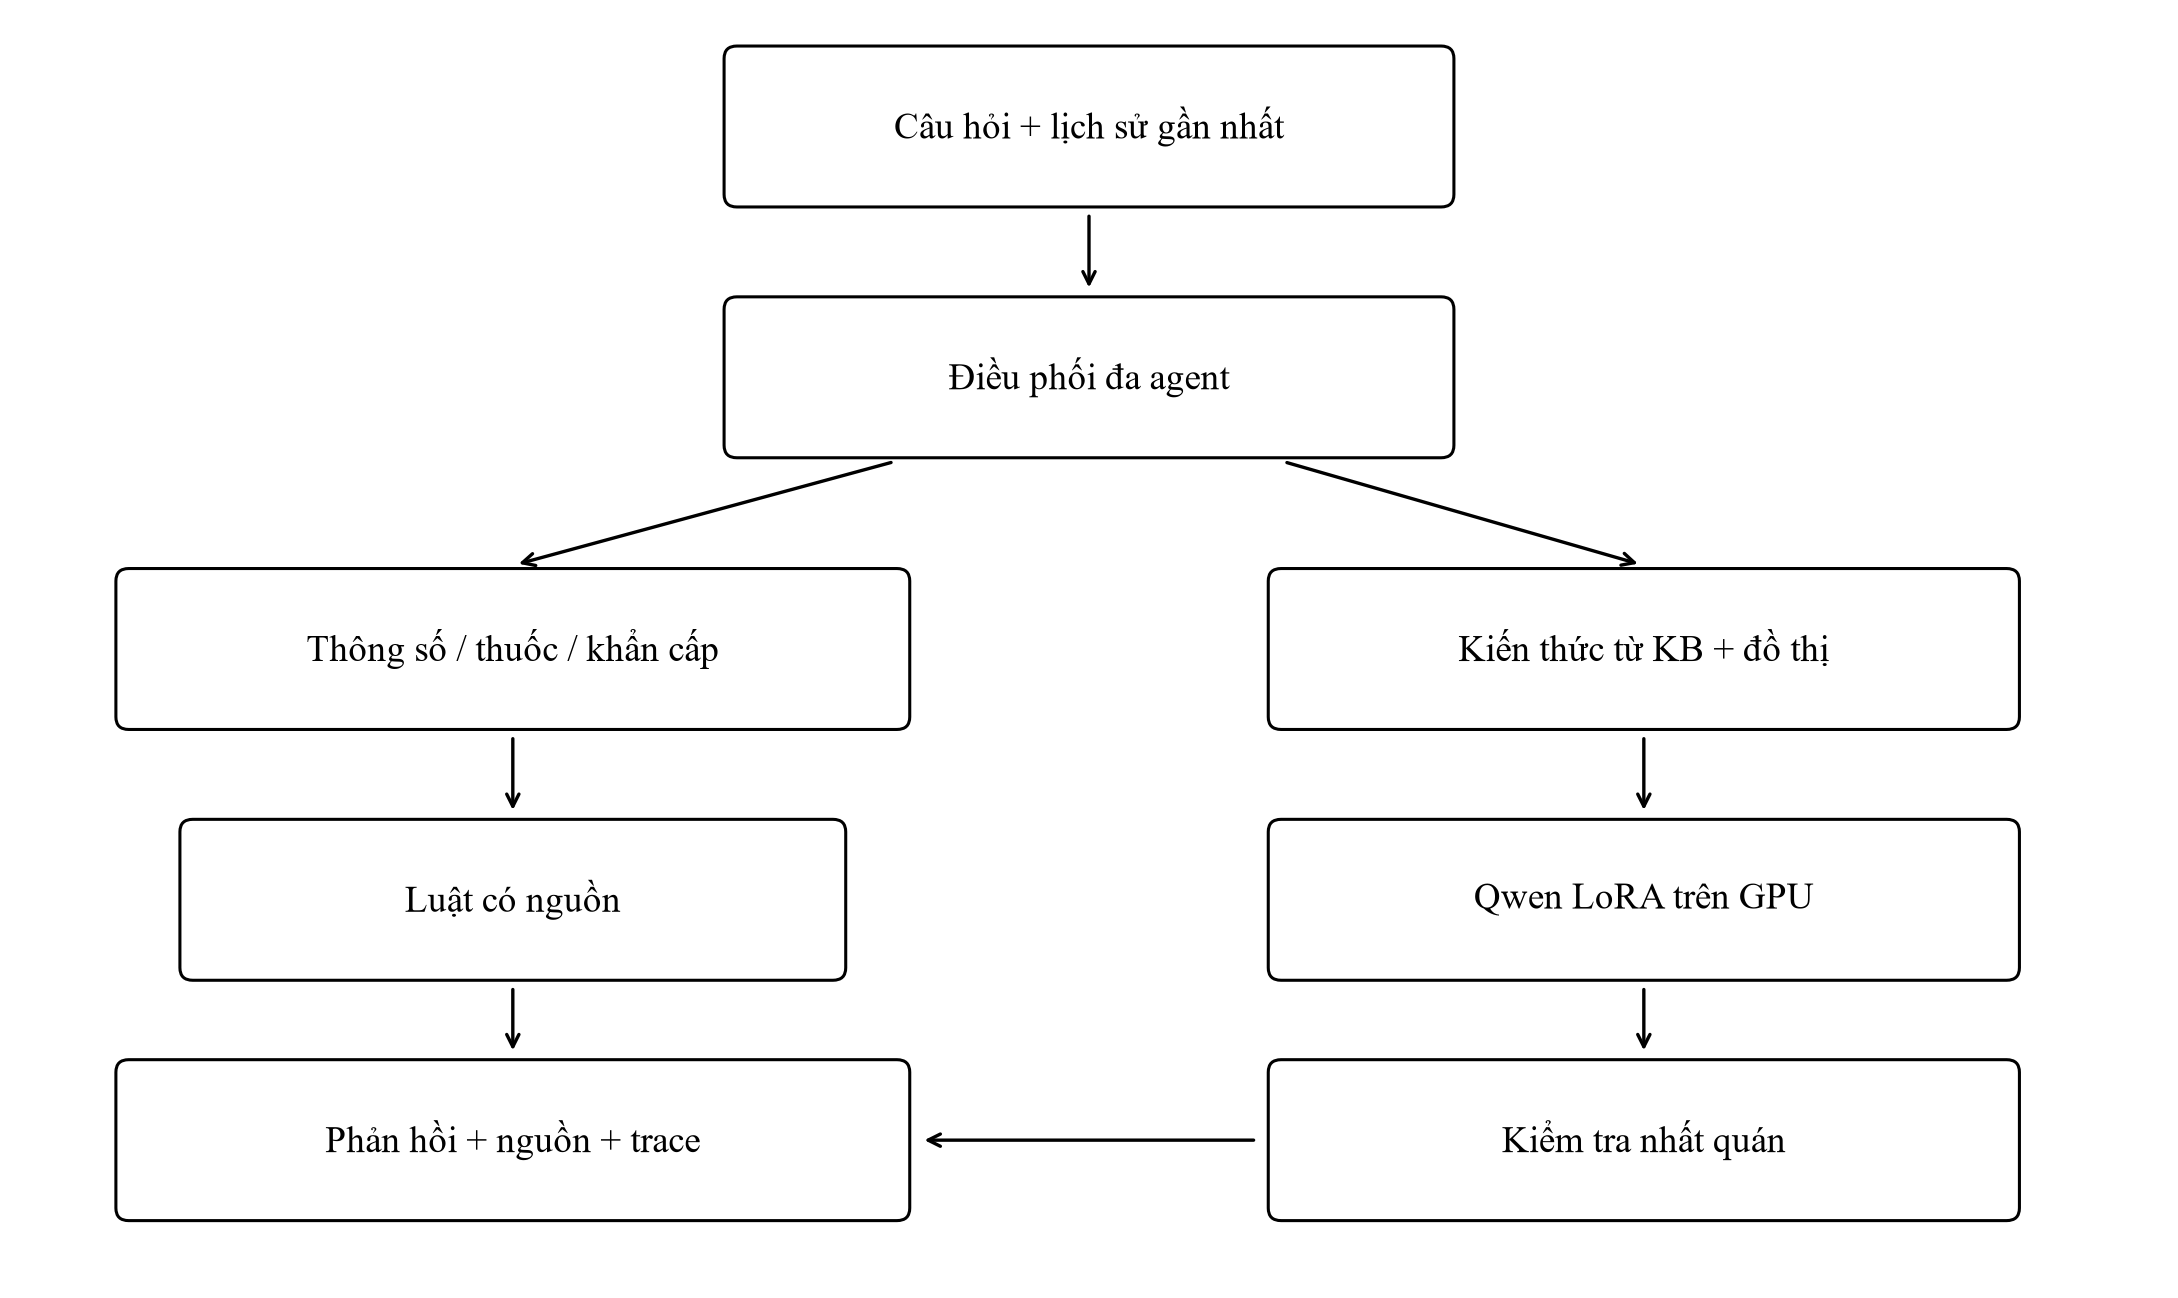
\includegraphics[width=\linewidth]{figures/local_architecture.png}\caption{Luồng xử lý tại máy cá nhân; phản hồi không đạt kiểm tra quay về nội dung KB.}\end{figure}
Điều phối xác định loại yêu cầu, truy xuất đoạn KB và gửi thông điệp đến agent ngôn ngữ cục bộ khi phù hợp. Agent kiểm chứng đối chiếu mã trích dẫn, số liệu và một số biểu thức không được phép trước khi chuyển câu trả lời ra giao diện. Nếu tải mô hình thất bại hoặc bản sinh không đạt kiểm tra, hệ thống trả về nội dung KB và ghi nguyên nhân trong trace.

Câu chứa thông số, câu về thuốc và tình huống khẩn cấp được ưu tiên xử lý bằng luật có nguồn. Qwen không được tự quyết định liều thuốc hay xác nhận bệnh. Bộ kiểm chứng hiện tại là bộ lọc nhất quán, chưa kiểm tra được mọi sai lệch ngữ nghĩa. Lịch sử gần nhất hỗ trợ diễn đạt nối tiếp; lịch sử gửi từ trình duyệt không phải bộ nhớ bền vững giữa các phiên.
\subsection{Huấn luyện lại bộ nhận diện ý định}
Bên cạnh LoRA, project huấn luyện một bộ định tuyến câu hỏi tiếng Việt bằng TF--IDF ký tự và hồi quy logistic. Bộ ví dụ gốc có 64 câu train và 16 câu test; sau khi bổ sung các cách hỏi về ăn uống, trái cây, vận động, thuốc, theo dõi, huyết áp, HbA1c và câu ngoài phạm vi, tập có 112 câu train và 32 câu test. Các câu test không được đưa vào bước fit. Trên tập test nội bộ này, accuracy đạt 93,75\% và macro-F1 đạt 0,937. Mã, dữ liệu, checkpoint và dự đoán từng câu nằm tại \path{scripts/train_intent.py}, \path{data/intent_expansion.json}, \path{models/chat_intent.joblib} và \path{results/intent_evaluation.json}.

Tập ví dụ do project tự viết, cùng chủ đề và một số từ khóa xuất hiện ở cả hai tập; đây là phép thử định tuyến hẹp, không phải đánh giá hội thoại ngoài miền. Bộ này không cập nhật trọng số Qwen và không cải thiện độ chính xác của hai mô hình dữ liệu bảng. Các tình huống xã giao, thông số, thuốc và khẩn cấp vẫn có luật ưu tiên.
\section{Tái lập và vận hành}
Chạy \path{experiments/local_qwen/train.py} bằng môi trường \path{.venv-llm} để tạo checkpoint, log loss và phản hồi kiểm thử. Adapter dùng để chạy được đóng gói tại \path{models/qwen_adapter}; checkpoint huấn luyện gốc nằm tại \path{.local-training/qwen-lora/best}. Mô hình nền và cache được lưu ngoài Git vì dung lượng lớn. Sau khi có đủ tệp, chế độ suy luận đặt biến offline để không tải tài nguyên từ mạng.

Khởi động bằng \path{run-local-qwen.ps1}, giữ cửa sổ tiến trình hoạt động và mở:
\productlink{Demo Qwen cục bộ}{http://localhost:8766}
Địa chỉ này chỉ dùng trên máy đang chạy dịch vụ. Neo4j cục bộ phục vụ đồ thị; chức năng hội thoại dựa trên KB vẫn có cơ chế dự phòng khi không kết nối được đồ thị.

\begin{figure}[H]\centering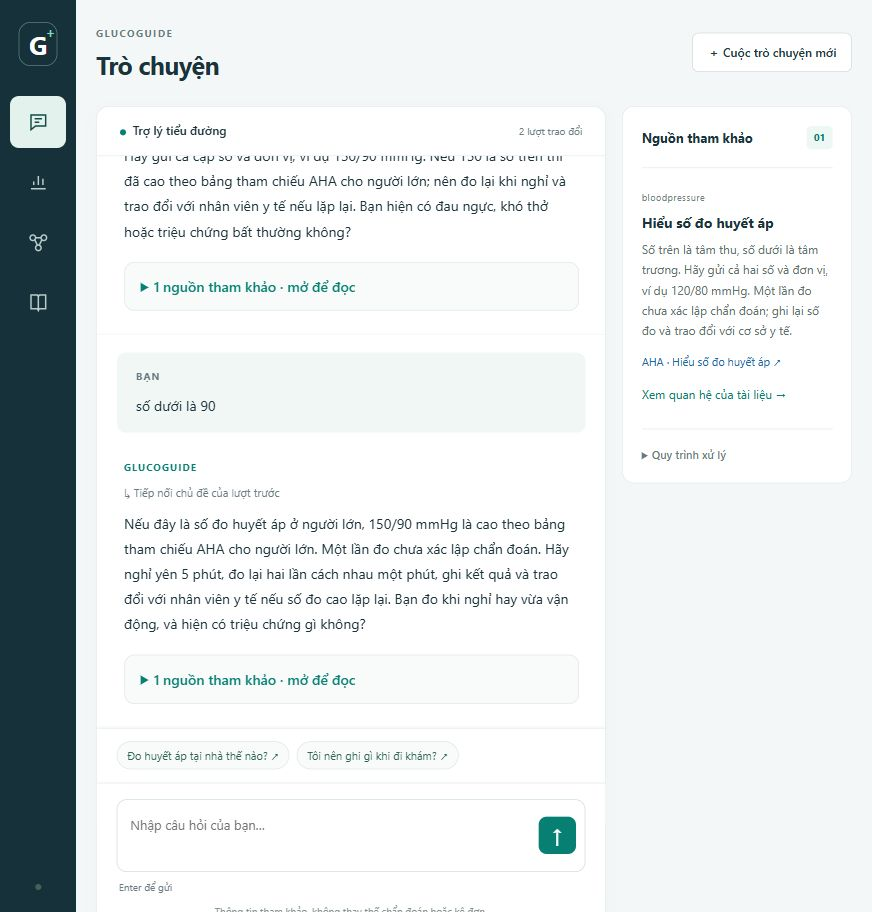
\includegraphics[width=.78\linewidth,height=.58\textheight,keepaspectratio]{demo-local-context.png}\caption{Kiểm tra hai lượt trên web local: hệ thống ghép thông tin bổ sung thành cặp số 150/90. Trường hợp này do luật hội thoại xử lý, không phải đầu ra tự do của Qwen.}\end{figure}

\subsection{Kiểm thử tích hợp trên web local}
Tám kịch bản qua HTTP đã chạy thành công: chia bữa ăn và định nghĩa tiểu đường dùng Qwen LoRA; chào hỏi, huyết áp, bổ sung số dưới, thiếu đơn vị, yêu cầu liều thuốc và bất tỉnh dùng luật. Mã phản hồi ghi rõ thành phần tạo câu trả lời. Nhật ký tại \path{results/local_qwen/runtime_checks.json} lưu yêu cầu, phản hồi, thông điệp giữa các agent và thời gian đo. Các kiểm tra bổ sung gồm 37 tình huống chatbot và 7 điều kiện của bộ kiểm chứng/MessageBus. Đây là tập kiểm thử chức năng hữu hạn, không phải chứng nhận đúng với mọi cách hỏi.

Một chuỗi kiểm thử bổ sung gồm câu hỏi chia bữa ăn, lời chào, lời phàn nàn, câu hỏi về xét nghiệm và câu hỏi tiếp ``là sao. Ban đầu, câu xã giao và câu hỏi ngắn bị truy xuất theo độ giống văn bản rất yếu, kéo các đoạn không cùng chủ đề vào câu trả lời. Phiên bản sửa nhận diện lời phàn nàn như một lượt giao tiếp; câu yêu cầu giải thích lại được gắn với câu hỏi chuyên môn gần nhất và chỉ đưa các đoạn nguồn thuộc chủ đề đó. Kiểm thử hồi quy xác nhận hai lượt này không còn lẫn tài liệu về bữa ăn, huyết áp hoặc mỡ máu.
\begin{figure}[H]\centering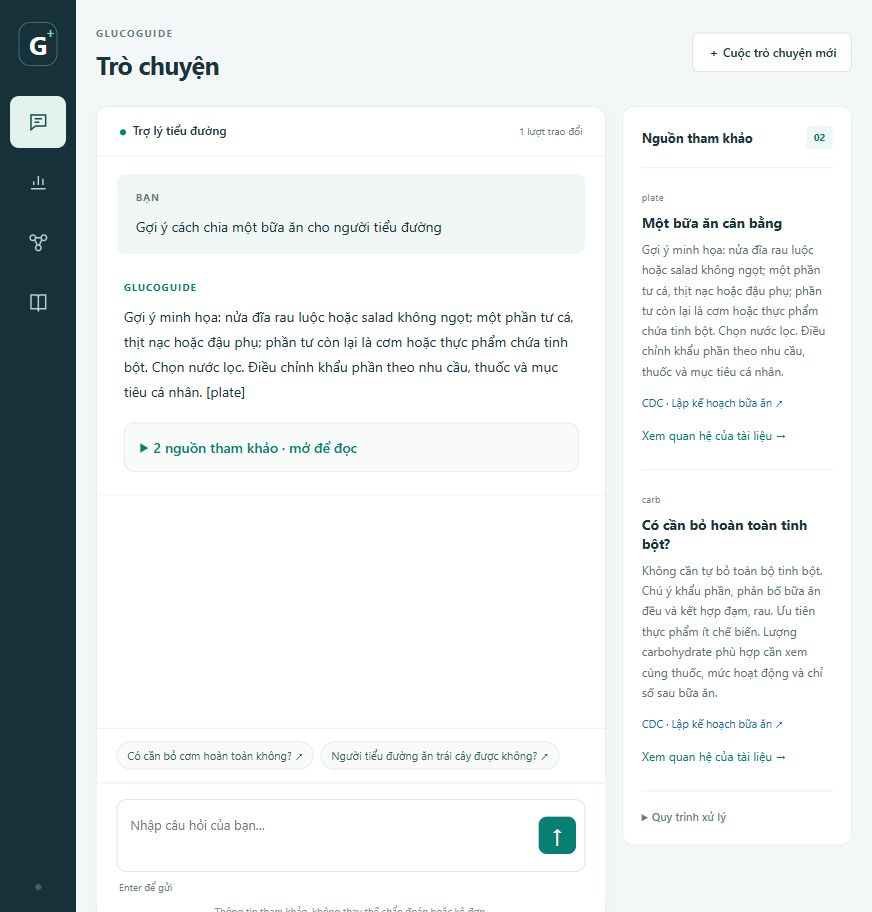
\includegraphics[width=.78\linewidth,height=.58\textheight,keepaspectratio]{demo-local-qwen.png}\caption{Phản hồi Qwen LoRA trên web local sau huấn luyện, kèm các đoạn nguồn truy xuất.}\end{figure}
